
\paragraph*{}
The agents we chose to populate our arsenal were picked from the ANL2022 contestants and CSE2310 agents (available \href[]{https://tracinsy.ewi.tudelft.nl/pubtrac/GeniusWebThirdParties/browser/ANL2022}{here} and \href{https://tracinsy.ewi.tudelft.nl/pubtrac/GeniusWebThirdParties/browser/CSE3210}{here} respectively) based on individual performance and group versatility. Agents' performance was of course a factor, but versatility (in the sense that agents' strategies should vary) was also considered, since similarities in strategy would mean similar strengths and weaknesses, and thus choosing between them wouldn't make much of a difference.
The agents that comprised our arsenal were the following:

\begin{enumerate}
    \item \textbf{GEA\_Agent:} Uses a simple opponent model and a decision tree to find good offers. Uses learning to classify opponents. Implements the BOA framework \cite{BOA_paper}. See \href[pdfnewwindow]{https://tracinsy.ewi.tudelft.nl/pubtrac/GeniusWebThirdParties/browser/ANL2022/gea_agent/ANAC 2022 GEA report.pdf}{here} for more information.

    \item \textbf{DreamTeam109:} The winner of ANL 2022 in both individual utility and social welfare. Also implements the BOA framework. Learns the best time to start compromising versus each opponent. See \href{https://tracinsy.ewi.tudelft.nl/pubtrac/GeniusWebThirdParties/browser/ANL2022/dreamteam109_agent/DreamTeam109 ANL2022 Agent Strategy.pdf}{here} for more information.

    \item \textbf{Agent007:} Uses frequency-based opponent modeling \cite{HardHeaded}. Came in second in the social welfare category of ANL 2022. Observed to achieve very high utilities in experimental tournaments run while exploring the alternatives. % Its function remains a mystery, since no report is available we haven't read the code. % TODO: remove!

    \item \textbf{TemplateAgent:} Given from ANAC as an example of an agent implementation to help competition participants. Acts like a hardliner for the best part of a negotiation session and starts conceding linearly close to the end. As a result of the hardliner behavior, many opponents may accept its demands before the conceding period begins in order to avoid a disagreement. Observed to perform well in various experiments as well.

    \item \textbf{Agent33:} Alexander The Great. Jesus Christ. Larry Bird.
    % Korydallos Correctional Facilities.
    The number 33 just seems to be inexplicably linked with greatness, and who are we to deny the ways of the universe?	% TODO: ti kanoume edw lol
\end{enumerate}
We refer to agents that TheNegotiator uses as \emph{strategy agents}.

\paragraph*{}
The inquisitive and skeptic reader might have had some thoughts along the lines of \quotes{those agents were made to participate in competitions, not to be used by other agents. Was that not a problem?} \textendash \ and they would be correct. In order to use readily available agents as part of our arsenal we had to make some adjustments to their code. We made the modification process very simple (2 lines of code per agent) since changing arsenal configuration was a crucial part of our process and we had to keep its overhead as small as possible.

\paragraph*{}
The fact that the agents were made to participate in the same competition meant that there was a lot of uniformity in their design, and thus they could all be interacted with in the same way. Since they were all designed to communicate with the same machinery (henceforth referred to as the \emph{protocol}), we had to \emph{be the protocol} as far as they were concerned: we had to do everything the protocol would do if they were in a real tournament. % TODO: what is a protocol? how does the reader know?
This begs the question of \emph{what does the protocol do}. Basically the process is as follows: it creates the agent (instantiates its class), passing only the path to its storage directory as a constructor argument. The rest of the interactions take place through a method that all agents have to implement, named \texttt{notifyChange} that is called by the protocol whenever something happens, and contains the agent's logic as to how to handle each event. The possible event types are the following:
\renewcommand{\arraystretch}{1.5} % Adjust the value as needed
\begin{longtable}{l p{290pt}}

    \texttt{Settings}: & Happens only once at the start of the negotiation session. Informs the agent of the domain and its profile. \\

    \texttt{Finished}: & Happens only once at the end of the negotiation session. The agent must then free its resources. \\
    
    \texttt{ActionDone}: & Happens each time an agent acts. This is the way agents learn the actions of their opponents. \\
    
    \texttt{YourTurn}:	& Means that the agent must tell the protocol if it accepts the opponent's offer or extend one of its own. \\

\end{longtable}

\paragraph*{}
The way in which one would mimic the protocol is quite straightforward. When we are notified of a new negotiation session (through a \texttt{Settings} event) we will select the appropriate agent and instantiate it, giving it a directory (inside what the protocol gave us) to use for its purposes. Every other event can just be passed to the strategy agent % TODO: to xoume orisei pouthena ?!
as-is, and it will do its thing. However, in the case of a \texttt{YourTurn} event, the way the agent sends its action to the protocol is not so straightforward, and thus requires a more intrusive approach. % TODO: intrusive in the sense that we intrude its code and alter it, better way to say that?

\paragraph*{}
The way the agent sends its action to the protocol is the following (see \cref{fig:protocol-agent_connection}):
\begin{enumerate}
    \item When the agent is created, the protocol \emph{connects} with it: a two way socket-like connection is established, that can be used to exchange data between them. \footnote{Agents are actually just listeners on this connection, and \texttt{notifyChange()} is just the callback function.}
    
    \item When a \texttt{YourTurn} event is received and the agent's logic has produced an action, it is sent to the protocol through that connection.
\end{enumerate}
Luckily, the only time agents may need to send data to the protocol is at the end of a turn. This means that we are free to override this connection from the agent's side and intercept any data going through it.

\begin{figure}[H]
\centering
\framebox{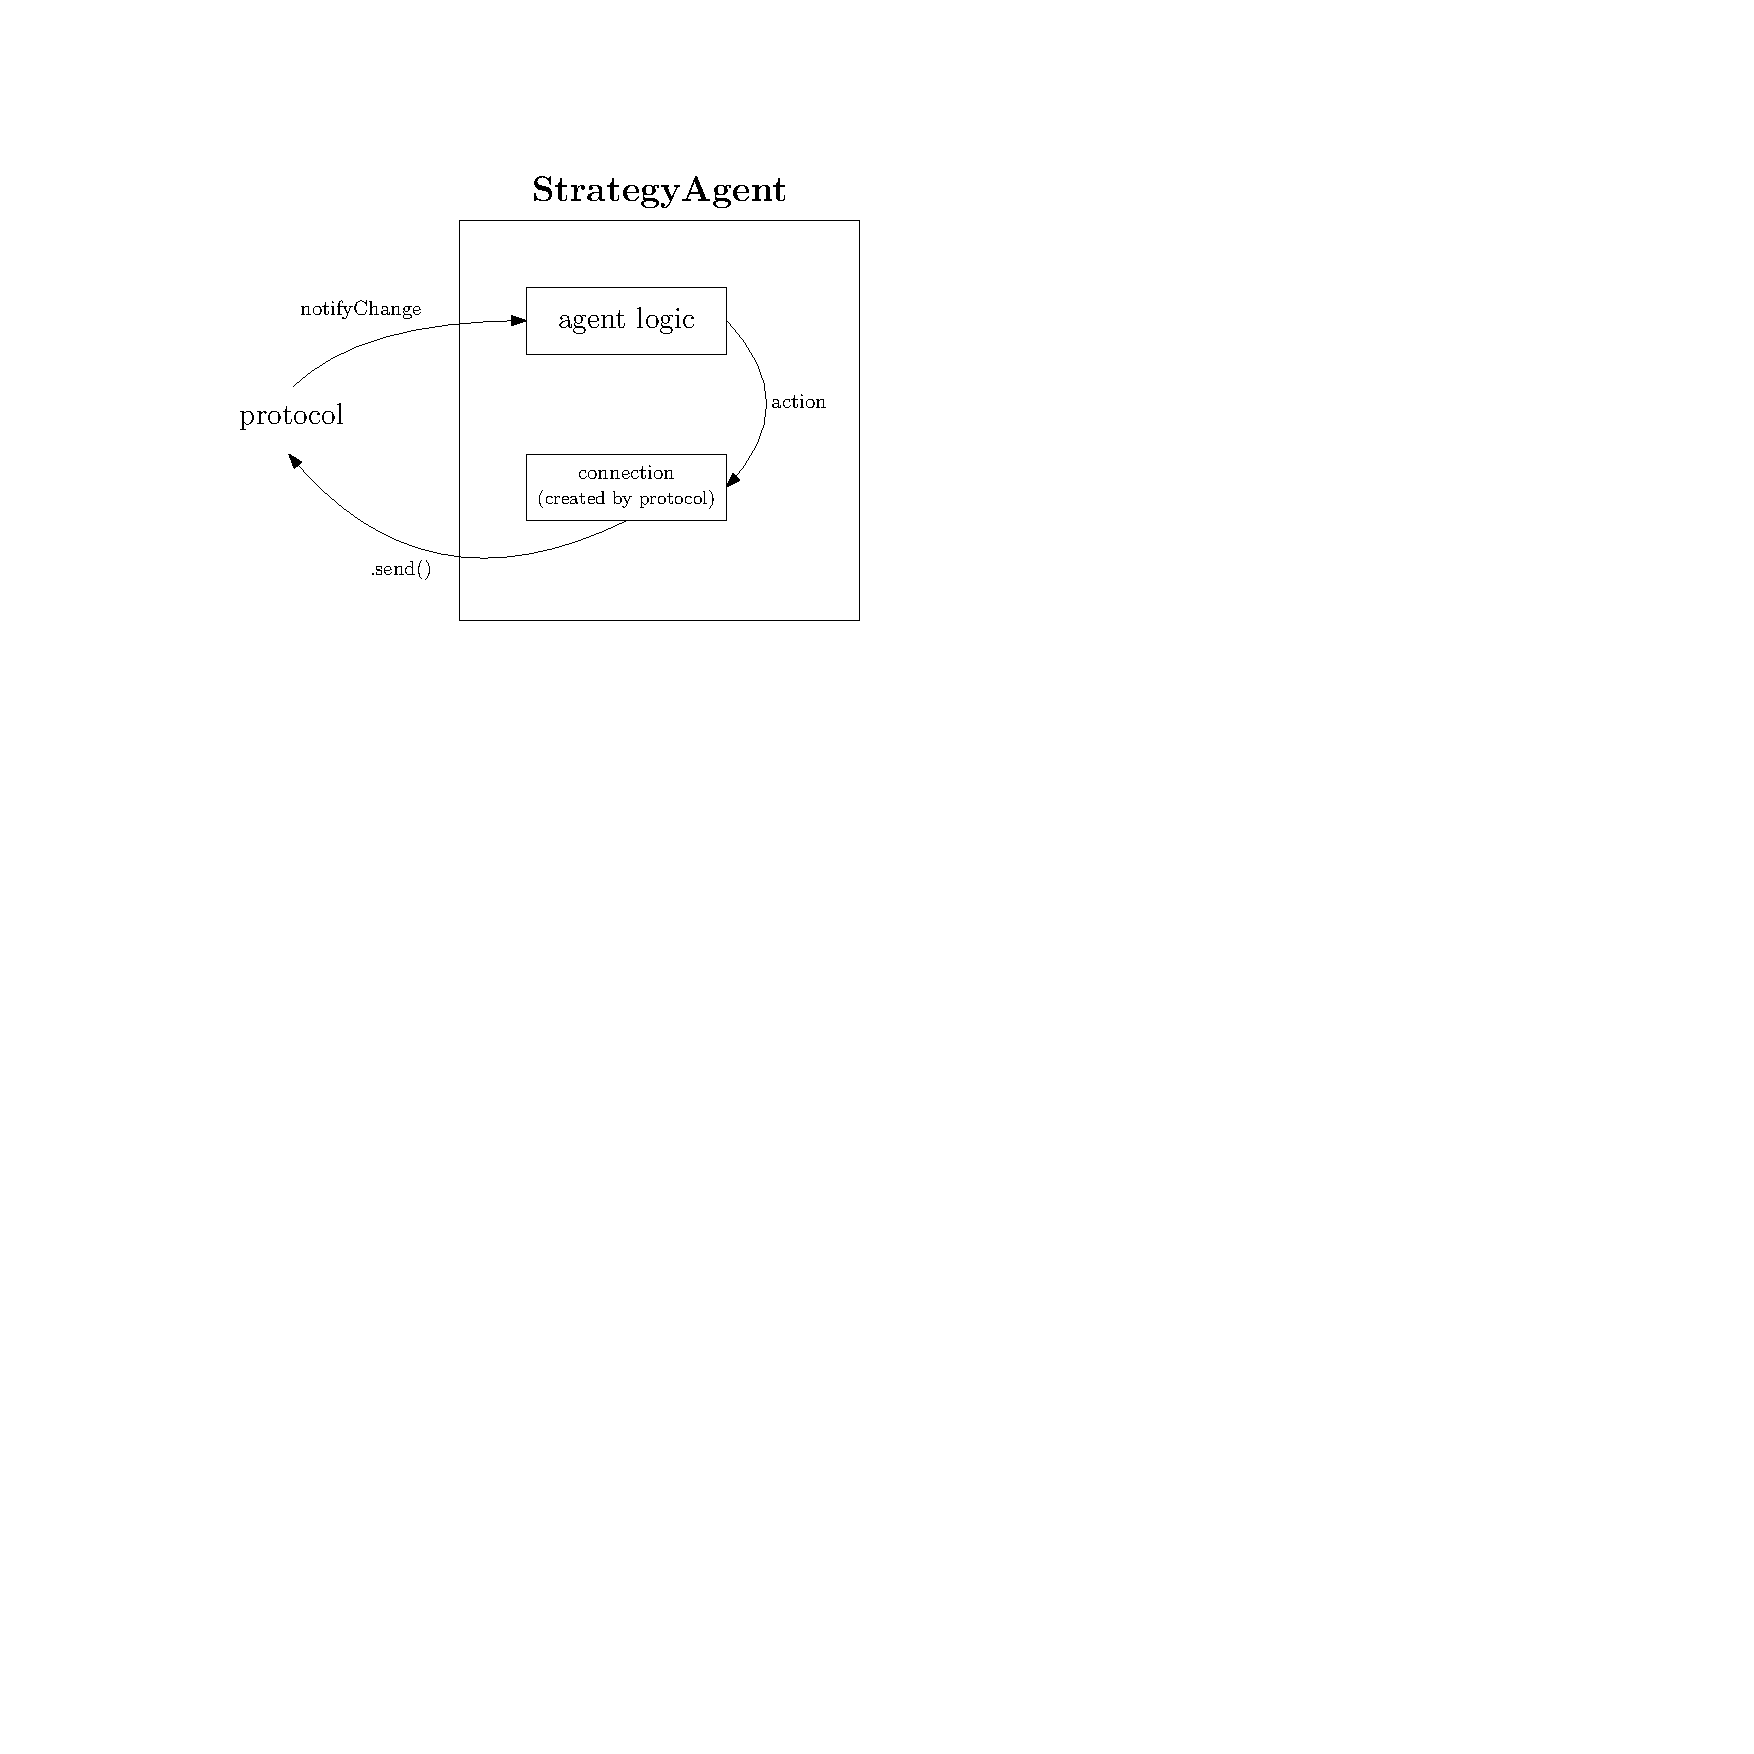
\includegraphics[scale=0.5, page=1]{mixin_explainer.pdf}}
\captionsetup{justification=centering}
\caption{The communication between the protocol and a generic agent}
\label{fig:protocol-agent_connection}
\end{figure}


% TODO: this here paragraph is up for review
\paragraph*{}
Unfortunately the way the protocol establishes this connection is quite complicated, so much so that using it to establish a such a connection between TheNegotiator and the strategy agent is neither guaranteed to work nor worth the hustle. % TODO: h zwh me ekane hustla
Our approach (see \cref{fig:agent-agent_connection}) was extremely simple, and based on the fact that the connection is just an attribute of the agent, and as such can be overwritten easily.

\paragraph*{}
We created a \texttt{CustomConnection} class that mimics the connection at the agent's end. Objects of this class are linked with a proxy when created, and when \texttt{send()} is called, they just copy that data to an attribute of the proxy.	% TODO: attribute or class variable?

\paragraph*{}
In order to \quotes{plant} the custom connection in the agents we want to use, we created the \texttt{ConnectionInterceptMixin}, that offers two methods. One is used to override the connection's \texttt{get()} method and return the custom connection instead of the real one. The other one lets TheNegotiator set itself as the proxy, giving it access to all the data sent through that connection. All one then has to do to make an agent usable by TheNegotiator is make it include the \texttt{ConnectionInterceptMixin}.

\begin{figure}[H]
\centering
\framebox{\includegraphics[scale=0.5, page=3]{mixin_explainer.pdf}}
\captionsetup{justification=centering}
\caption{The communication between the protocol and TheNegotiator using a strategy agent}
\label{fig:agent-agent_connection}
\end{figure}

